%!TEX root = main.tex

\documentclass[main.tex]{subfiles}

\begin{document}

\chapter{Background}
Fill me in later.
In this chapter we give an overview of what the slide guitar is as well as an introduction to the theoretical framework of digital waveguides which form the basis for the synthesis model developed in this thesis. After these ideas have been covered, the development of a basic outline for a slide guitar model will be developed. This will be a basic overview as more details will be developed later in the thesis. The end of provides an overview and comparison of more recent slide guitar modeling developments.

\section{What is the slide guitar?}
ADD SOMETHING ABOUT GUTIAR ANATOMY, INCLUDE THE DEFINTION OF SCALE LENGTH

One of the more unique methods of playing guitar is an approach referred to as “slide guitar”. This consists of using a smooth rigid tube (the slide) to control the length of the string, instead of the frets and fingers. The slide acts as a string termination and influences the vibration of the string by creating a new load termination in between the nut and the bridge \citetwo{evangelista_physical_2012}. This allows unique articulations and pitch inflections to be generated as the player is no longer constrained to the pitches provided by the fret locations. Additionally, the interaction of the slide’s surface with that of the string adds a new timbral component related to the slide’s velocity \citetwo{pakarinen_virtual_2008}. Figure \ref{fig:acoustic_chrome} shows a player using a chrome slide on an acoustic guitar.

\begin{figure}[h]
    \centering
    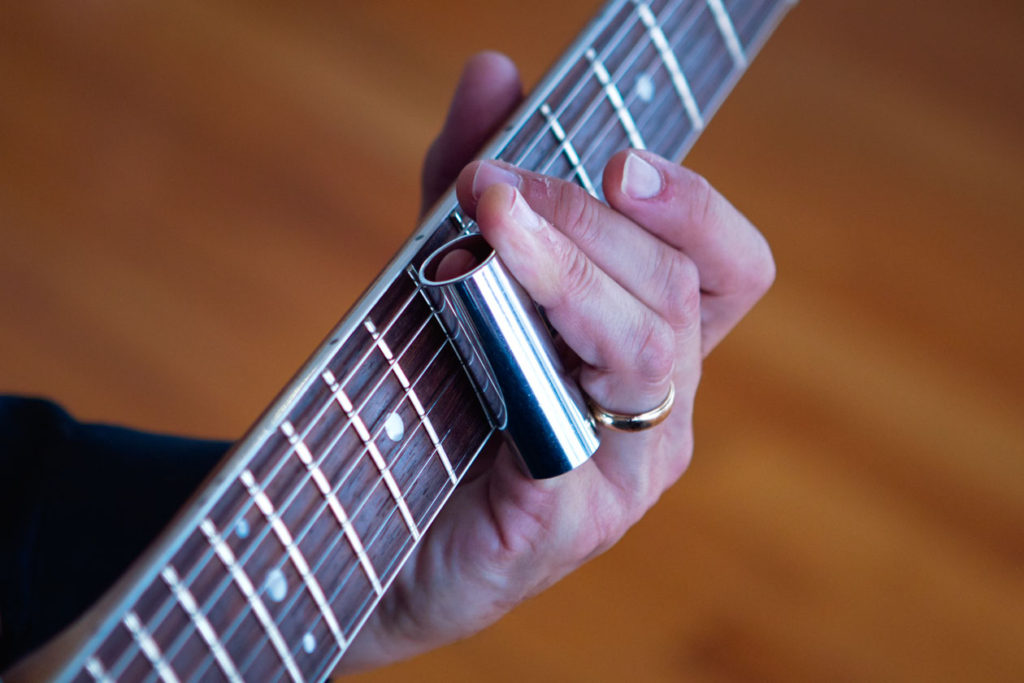
\includegraphics[scale=.30]{./images/pictures/Slide-guitar-1024x683.jpg}
    \caption{An acoustic guitar played with a chrome slide}
    \label{fig:acoustic_chrome}
\end{figure}

In the case of wound strings, this adds two new sounds. The first is a time-varying harmonic component due to the interaction of the slide with the spatially periodic pattern of windings on the string’s surface (inherent in a wound string’s construction) \citetwo{pakarinen_analysis_2007}. The second component is due to the stimulation of the string’s longitudinal modes as the slide introduces disturbances in this direction when it impacts the ridges of the windings. As the slide does not provide sufficient force to change the longitudinal length, the longitudinal mode frequencies are static, regardless of the motion of the slide \citetwo{pakarinen_analysis_2007}. Figure \ref{fig:slide_string_zoom} shows a close up of a slide interacting with a wound string.

\begin{figure}[h]
    \centering
    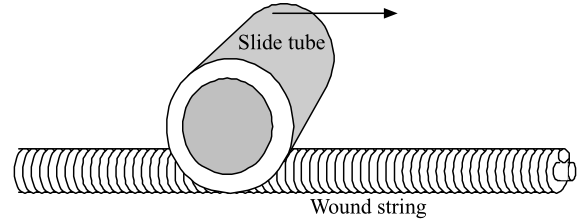
\includegraphics[scale=1]{./images/pictures/slide_wound_string_zoom.PNG}
    \caption{Close up of a slide on wound string}
    \label{fig:slide_string_zoom}
\end{figure}

Slides are traditionally made from ceramic or metal and unwound strings are made with metal \citetwo{bhanuprakash_finite_2020}. Figure \ref{fig:slide_types}. These are smooth/polished materials. Correspondingly, the coefficient of friction between the string and slide is comparatively much lower than in the wound-string case. Unwound strings also have a uniform surface, lacking the ridges created by windings which a slide impacts while traveling the length of the string. This drastically reduces the coupling between the slide and the unwound string from a longitudinal standpoint, with the result that the longitudinal modes are not audible. As a result, the contact sound generated for unwound strings is more akin to white-noise scaled by the slide velocity and lacks a harmonic component. \citetwo{pakarinen_virtual_2008}. 

\begin{figure}[h]
    \centering
    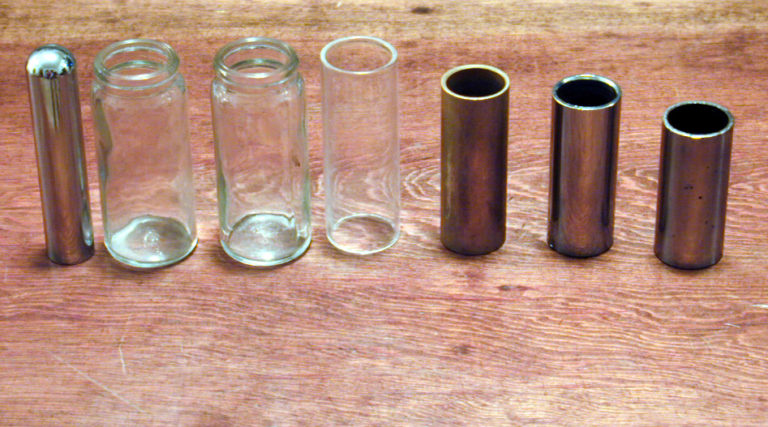
\includegraphics[scale=.35]{./images/pictures/Slide-guitar-different-slides-768x427.jpg}
    \caption{A selection of slides made from different materials}
    \label{fig:slide_types}
\end{figure}

\section{What is physical modeling and digital wave guides?}

Physical modeling is a discipline which attempts to recreate physical phenomena using computational algorithms. There are many different approaches to this, however one of the most popular and well developed is the technique of digital waveguides (DWG). As the name would imply, this approach uses algorithms and data structures to mimic the method by which waves propagate throughout a medium. It is an extremely computationally efficient technique which has been incorporated into many different commercial synthesizers.

\subsection{Fundamental Components}

Three of the fundamental components of digital waveguide models are: digital filters, digital delay lines and fractional delay lines. The inter-connection of these different components can model a variety of linear wave propagation phenomena. Incorporating different noise sources and initialization waveforms facilitates an enumerable number of different sound synthesis algorithms.

\subsubsection{Digital Filters}

Conceptually digital filters are extremely similar devices. They merely add scaled time delayed versions of their inputs and outputs. Through various combinations of delay amounts and scaling, a range of different frequency domain effects can be achieved. They are linear systems themselves, which is useful as the entire branch of LTI systems is now made available to the algorithm designer.

They come in two varieties: FIR and IIR filters. FIR filters consist of only delayed and scaled copies of the input signal while IIR filters incorporate the out of the filter via a feedback line. This ultimately is what gives rise to the "infinite" aspect of their name.

They do suffer from the nature of transients. These occur whenever there is a change in the coefficients associated with a filter structure as well as when the input changes from steady state. FIR filters have a transient whose length corresponds to the length of the filter. IIR filters pose more of a problem in this instance as their feedback lines ultimately cause the transient to propagate for a much longer time (depending on their coefficients).

\subsubsection{Digital Delay Lines}

One of the fundamental components of DWG based modeling is the digital delay line. It's main purpose is to provide a computational model of the physical traveling wave. It represents spatial samples of the physical medium which is being modeled. The physical distance between each spatial sample corresponds to the distance a wave travels during one sampling period. Mathematically, this can be expressed in the following equation:

\begin{equation}
    X_s = T_s \times c
\end{equation}
where $T_s$ is the temporal sampling period, $c$ is the wave propagation speed in the particular media being modeled and $X_s$ is the spatial sampling period.
An inherent limitation to digital delay lines is the fact that the fundamental unit of discretization in the time-domain is the sample. Signals can only be delayed integer numbers of samples with these. In many physical modeling applications, this is a limitation due to the fact that the physical world and its associated problems often require knowing a physical quantity which doesn't correspond to a sampling location.

\subsubsection{Fractional Delay Components}

Due to the limitations of purely integer based delay-lines, as mentioned in the end of the previous section, various approaches have been developed in an attempt to approximate the signal values in between samples. These approaches can be referred to as fractional delay lines. These approaches are implemented using digital filters.

One popular approach to fractional delay line implementations is the Lagrange approach. In this technique an FIR filter is used where the filter coefficients implement Largange interpolation to allow for sub-sample accuracy. They are also generated via the maximally flat criteria. The order of the filter determine the order of the polynomials involved. With an order of N = 1, linear interpolation is achieved. Adjusting the order of the filter allows you to have more control over its frequency response and phase delay. These benefit from a constant phase delay under certain conditions.

Another popular approach is referred to as Thiran interpolation. The basis of these is the all-pass filter.

\subsection{Applied to String Modeling}

In string modeling the main variable of interest is often the transverse displacement of the string at various spatial locations across different points. In combination with the characteristic impedance of the string, various acoustic quantities can be derived. Accordingly, the digital wave guide model of a string consists of a digital delay line. The terminations can be represented by simple reflection coefficients. The effects of the bridge/body connection can be modeled using a loop filter to represent the appropriate losses.

Add some stuff about how controlling the string length changes the fundamental frequency.

Also add some stuff about how the length of the delay line maps on to the length of the signal.

Add some stuff about how the development of the string model has been researched quite a bit, especially computational approaches to it.

Add some stuff about how the length of the string controls the pitch, from the previous paper on the development of a guitar synthesizer.

\section{Development of a basic slide guitar digital wave guide model}

The slide guitar model which serves as the basis for this thesis originally comes from a computer music journal described in \citetwo{pakarinen_virtual_2008}. The basis for this model is the single-delay line string as described earlier with an additional component to model the slide/string surface interactions as well as energy compensation gain block. The model is shown in figure \ref{fig:original_DWG}. A special loop filter was also designed where the coefficients used were generated by recording the output of a professional player, picking various notes across the length of the neck.

\begin{figure}[h]
    \centering
    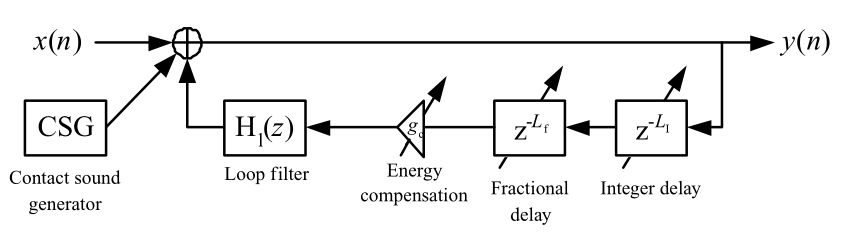
\includegraphics[scale=.75]{./images/pictures/SDL_slide_model.PNG}
    \caption{Slide guitar DWG model from \citetwo{pakarinen_slide_2008}}
    \label{fig:original_DWG}
\end{figure}

All the components in the model are effectively controlled by the relative length of the string. This is depicted as $L(n)$ in the figures from the original paper. Naturally, this maps onto the notion of how a guitar works in general. Given that frets normally change the relative length of the string, with the fret spacing corresponding to the tuning system the guitar is designed for (12-TET being the most common), the relative length of the string being modeled is a natural control signal. The other main command/method of interacting with this model is via a "pluck" where the waveform in string model is initialized and the simulation begins to run. In the fretted paradigm of playing this $L(n)$ signal would be restricted to a finite set of values based on the number of frets of the guitar as well as their locations. In the slide guitar model, this is not the case. We now have an entire continuum of pitches to explore so theoretically the $L(n)$ could take values on the interval $(0,1]$. However, the limitations on the valid values are imposed by configurations of the constituent signal processing blocks (as will be discussed later in the thesis).

\subsection{Energy Compensation}

Talk about the energy compensation block here and the limitations and everything on it. Also, what it fundamentally serves to do.

\subsection{Loop Filter}
Add stuff in here about the loop filter, its coefficients, how they were extract and interpolated as well as what the loop filter fundamentally serves to emulate. Add the equations for the polynomial approximations.

\subsection{CSG Development}

\begin{figure}[h]
    \centering
    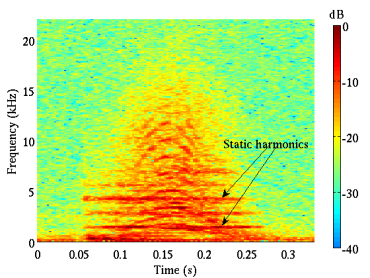
\includegraphics[scale=1]{./images/pictures/finger-noise-spectrogram.png}
    \caption{Spectrogram of handling noise generated by sliding a finger on a wound guitar string from \citetwo{pakarinen_analysis_2007}}
    \label{fig:finger_noise_spectrogram}
\end{figure}


The handling noises based on wound string and finger interactions have previous been investigated in \citetwo{pakarinen_analysis_2007} and \citetwo{penttinen_model-based_2006}. The slide itself is slightly different, however the underlying framework developed by the finger noise analysis is extremely valid and can easily be adapted to the slide scenario. Hence, we will commence with the analysis of the finger noise first.

\subsubsection{Finger Noise Analysis}

Figure \ref{fig:finger_noise_spectrogram} shows the spectrogram of the noise generated by dragging a finger tip across the surface of a wound guitar string \citetwo{pakarinen_analysis_2007}. As can clearly be seen, there are two components to the sound. The first is a time-varying harmonic component which corresponds to the interactions of the finger surface with the spatially periodic windings which appear on the string. The second is a static component which is due to the longitudinal modes which are stimulated by the finger impacting the windings. Similar results have been shown in \citetwo{penttinen_model-based_2006} where the guqin, a fretless Chinese stringed instrument, was examined. We can think of the contact noises as consisting of an exicter and resonator part. The finger-string impacts generate the excitation while the longitudinal string vibrations act as the resonator.

An object moving along a wound string creates a harmonic force excitation to the string. This is velocity dependent and can mathematically be expressed as:

\begin{equation}
    F(t) = \left[\sum_k \delta(t-t_k)\right] \ast f(t)
    \label{eqn:harmonic_force}
\end{equation}

where $f(t)$ is the impulse response from a single finger-winding colision, $t$ is time, $t_k$ is the time instant where the $k$th impulse response is generated and $\delta$ is Dirac's delta function. Equation \ref{eqn:harmonic_force} indicates we can interpret the force as a periodic impulse train being filtered by the transfer function of a single finger-to-winding collision.

The next obvious question to ask, is how are the $t_k$ values established? To simplify, we can start by assuming the finger motion is a constant velocity. In this case $t_k$ can be expressed as:

\begin{equation}
    t_k = \frac{k}{n_w f_{speed}}
    \label{eqn:t_k}
\end{equation}
where $n_w$ represents the linear winding density of the string (winds per meter), $f_{speed}$ represents the finger tip speed (meters per second). The quantity $n_w f_{speed}$ has units of windings per second and represents the number of collisions which occur at each second. We can see that by either increasing the linear winding density or finger speed we have control over the frequency at which the impulse responses are generated. From there, it is not difficult to see that as the $n_w$ parameter is constant per string, the fundamental of the harmonics generated can be controlled by the speed at which the finger moves. The faster the finger moves, the shorter the period between impacts is and the higher the fundamental of the resulting wave worm. A time-varying finger velocity generates a time-varying harmonic signal where the periodic waveform corresponds to the impulse response of a single finger-to-winding impact.

This theory can easily be verified by observing the spectrum in figure \ref{fig:finger_noise_spectrogram}. In this figure the finger starts at rest, accelerates to reach its maximum velocity halfway through the slide, at which point it begins to decelerate as the slide comes to an end. The minimum and maximum values of frequency trajectories corresponding to the different harmonics illustrate the same behavior in this spectrogram. It is also interesting to note that these harmonics follow a differentiable trajectory so we can conclude that the finger velocity is also differentiable and contains no discontinuities (something which is necessary to note when attempting to synthesize sounds which mimic human players).

As shown experimentally in \citetwo{pakarinen_analysis_2007}, the amplitude of the harmonic noise component is linearly related to the slide velocity. This can also be intuited from a physical standpoint given that the higher the the finger velocity, the more momentum is transferred to the string during the collision. Assuming linearity, this would manifest itself as a velocity dependent scaling component associated with each $t_k$ value in equation \ref{eqn:harmonic_force}.

The other component from the sound, which has been labeled in figure \ref{fig:finger_noise_spectrogram}, is a static component due to the longitudinal modes of the string. The partial differential equation describing the longitudinal string motion, as derived in \citetwo{bank_physics-based_2006}, is the following:

\begin{equation}
    \mu \frac{\partial^2 \xi}{\partial t^2} = ES\frac{\partial^2 \xi}{\partial x^2} - 2R(f)\mu \frac{\partial \xi}{\partial t} + d(x,t)
    \label{eqn:longitudinal_PDE}
\end{equation}
where
\begin{itemize}
    \item $\xi(x,t)$ is the longitudinal displacement
    \item $E$ is Young's modulus
    \item $S$ is the string's cross sectional area
    \item $\mu$ is the linear mass density
    \item $R(f)$ is a frequency dependent frictional resistance
    \item $d(x,t)$ is the excitation force density
\end{itemize}
The wave propagation speed is $c_L = \sqrt{\frac{ES}{\mu}} = \sqrt{E \rho}$, where $\rho$ is the density of the material. Contrary to transverse modes, the longitudinal propagation speed for a wave does not depend on tension. If only one point of excitation exists, then the spatial force distribution can be approximated as: $d(x,t) = \delta(x_{exec})F(t)$ where $x_{exec}$ is the point of excitation.

As shown in \citetwo{pakarinen_analysis_2007} and \citetwo{morse_vibration_1981}, if an excitation force $F(t)$ is applied at $x_{exc}$, then the bridge force can be expressed as:

\begin{equation}
    F_b(t) = \frac{ES}{\mu L^2} \sum_{k = 1}^{\infty} \left[\frac{k}{f_k} e^{-t R(f_k)} \sin(2\pi f_k t)\right] \ast \left[ \sin\left(\frac{k \pi x_{exc}}{L}\right) F(t)\right]
    \label{eqn:bridge_force}
\end{equation}
where the longitudinal modal frequencies are $f_k = k \frac{c_L}{2L}$. Equation \ref{eqn:bridge_force} clearly shows that the force signal excites a set of parallel resonances where the excitation amplitude depends on $x_{exc}$. In general, $x_{exc}$ has a strong shape over the spectrum and in the cases where a mode as a node at the point, the harmonic will be eliminated. This theory was experimentally verified in \citetwo{pakarinen_analysis_2007}. 

This analysis was completed based on the interactions between a finger tip and a wound string. Extrapolating this to the more rigid slide object is quite intuitive. The physical properties of the string do not change, only the surface of the object interacting with the string. In terms of impact on the analysis, the only part of the equations which would change is the impulse response function $f(t)$ in equation \ref{eqn:harmonic_force}. This would now represent the impulse response of the slide impacting a single winding.

\subsubsection{CSG Model Development/Analysis}

The Contact Sound Generator (CSG) of the slide synthesis model can be seen as a discretization of the exciter-resonantor model developed in the previous section. Figure \ref{fig:original_CSG} shows a high-level signal flow diagram of the original CSG presented in \citetwo{pakarinen_virtual_2008}. 

\begin{figure}[h]
    \centering
    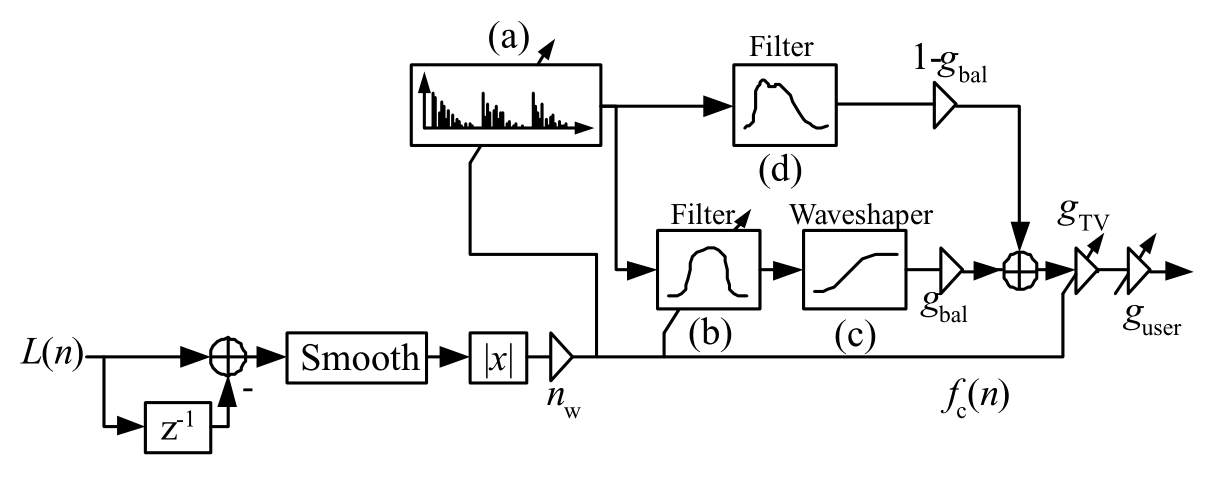
\includegraphics[scale=.50]{./images/pictures/CSG_original.PNG}
    \caption{CSG model from \citetwo{pakarinen_slide_2008}}
    \label{fig:original_CSG}
\end{figure}

A noise pulse train is chosen as the excitation signal, which is labeled as block $(a)$ in figure \ref{fig:original_CSG}. This choice is based on the assumption that the impulse response from a single slide-to-winding collision can be modeled as an exponentially decaying noise burst. Example noise bursts are shown in \ref{fig:noise_pulses}. The time-interval between noise pulses is controlled by the slide velocity as illustrated in equation \ref{eqn:t_k}. In a certain regard, the CSG can be viewed more as a periodic impact synthesis model more so than a frictional model, which matches with how the slide makes contact with the windings. The faster the slide moves, the denser the pulse train becomes, with some of the IRs overlapping depending on the decay rate associated with the string. The decay rates and correspondingly durations of the noise pulses are parameters associated with each different string thickness.

\begin{figure}[h]
    \centering
    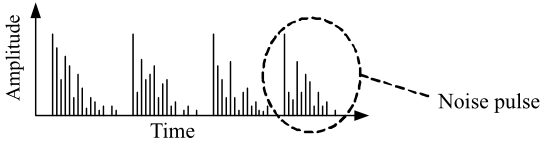
\includegraphics[scale=1]{./images/pictures/noise_pulses.PNG}
    \caption{Noise Pulses from \citetwo{pakarinen_slide_2008}}
    \label{fig:noise_pulses}
\end{figure}

At the lower-left branch of the CSG we have the control signal $L(n)$ coming in. This represents the relative length of the string. The first-order derivative of $L(n)$ is approximated to generate the relative slide-velocity. This is valid given that the position of the slide controls the relative length of the string. From there the signal runs through a block labeled "Smooth". This block in fact performs two operations. The first is a smoothing operation, which helps handle any discontinuities which arise during the differentiation process. This is necessary, as discontinuities rarely happen, if ever, while play slide guitar due to the human controlled nature of the slide motion. The second operation this block performs is interpolation in the case that the control signal runs at a different sampling frequency than the audio signals (as is often the case). The interpolation allows the constituent synthesis model processing blocks to adjust in a more natural/gradual way as well and helps avoid transients in digital filters. In this scenario we are filtering noise so this is not as much of a concern but good to be aware of in general.

After the slide velocity has been up-sampled to the audio rate, the absolute value is then taken to produce the slide speed. Given that the impulse response generated from the impact of the slide with a winding is agnostic to the direction the slide is traveling, this is a valid operation. After this the relative slide speed is multiplied by $n_w$, the linear winding density, to generate the control signal labeled $f_c(n)$. This signal mimics the relationships expressed in \ref{eqn:t_k}. Accordingly, it controls the firing rate of the noise pulse generator as well as scales the output via the gain block $g_{TV}$.

The output of the noise pulse generator goes to two different branches, each approximating a different aspect of the contact sound. The lower branch is a 2nd-order resonator filter followed by a waveshaper implemented via a hyperbolic tangent. The 2nd-order resonator has its center frequency controlled by the aforementioned $f_c(n)$ in order to extract the lowest time-varying harmonic from the noise source. The series-connection with the waveshaper creates the higher time-varying harmonics in a computationally efficient manner. The number of harmonics can be controlled via a scaling factor to the input of the hyperbolic tangent.

The upper branch serves to emulate the static longitudinal modes. The filter there is a 4th-order IIR which approximates the two most prominent longitudinal modes. The coefficients of the filter are dependent on the different string/slide combinations as the different slide materials interact with the windings in a different manner. The filter's responses have been approximated via linear predictive coding (LPC) \citetwo{pakarinen_virtual_2008}. The $g_{bal}$ controls the balance between the longitudinal modes and the harmonic contact sound components.

\section{Other Developments and Approaches}

\end{document}
